\setcounter{section}{2}
\setcounter{subsection}{1}
\setcounter{subsubsection}{2}
\setcounter{equation}{8}
\setcounter{figure}{1}

\subsubsection{Die metallische Bindung}
	Die metallische Bindung ist ähnlich zu der kovalenten, da sie ebenfalls durch die Überlappung der Wellenfunktionen der Elektronen zustande kommt. Im Gegensatz zur kovalenten Bindung sind die Elektronen jedoch \textbf{nicht} lokalisiert.
	Daraus ergeben sich folgende Eigenschaften für Metalle:
	\begin{itemize}
		\item Der negative Elektronensee der quasi-freien Elektronen einer Metallverbindungen kompensieren die Coulomb-Abstoßung der Metallionen.
		\item Metallverrbindungen haben eine hohe Packungsdichte mit Koordinationszahlen zwischen 8 und 12.
		\item $N$ Elektronen wechselwirken mit $N$ Atomen. Die Energieniveaus sind also $N$-fach entartet.
		\item Es entsteht eine Quasi-Kontinuum der Bänder.
	\end{itemize}

	Die Metalle der verschiedener chemischer Gruppen besitzen unterschiedlliche Eigenschaften:
	\begin{itemize}
		\item \textbf{Alkalimetalle (\ce{Li}, \ce{Na}, \ce{K}, \ldots) }\\
			Alkalimetalle besitzen halb gefüllte s-Schalen (\ce{Na}, $3\mathrm{s}^{1}$).\\
			Sie haben geringe Bindungsenergien von ca. \SI{1}{\electronvolt \per Atom}.
		\item \textbf{Erdalkalimetalle (\ce{Be}, \ce{Mg}, \ce{Ca}, \ldots):}\\
			Die s-Schalen sind vollständig gefüllt, jedoch überlappen sich 3s-Energieniveaus mit p-Niveaus.
		\item \textbf{Übergangsmetalle (\ce{Fe}, \ce{Co}, \ce{Ni}, \ldots):}\\
			Die inneren, teilweise gefüllten 3d Orbitale $3\mathrm{d}^{6,7,8}$ überlappen sich mit den leeren Orbitalen mit $n=4$ ($4\mathrm{s}^2, 4\mathrm{p}^{6}$).
			Somit tragen diese auch bei zu den kovalenten Bindungen der 3d-Orbitale. \autoref{fig:vl15_ueberlapp_orbitale} zeigt den Überlapp dieser Orbitale bei Nickel.\\
			Übergangsmetalle haben eine hohe elektrische und thermische Leitfähigkeit und weisen starke Lichtabsorbtion und -reflektion auf.
			Typische Bindungsenergien sind ca. \SI{4}{\electronvolt \per Atom}.
	\end{itemize}
	\begin{figure}[H]
		\centering
		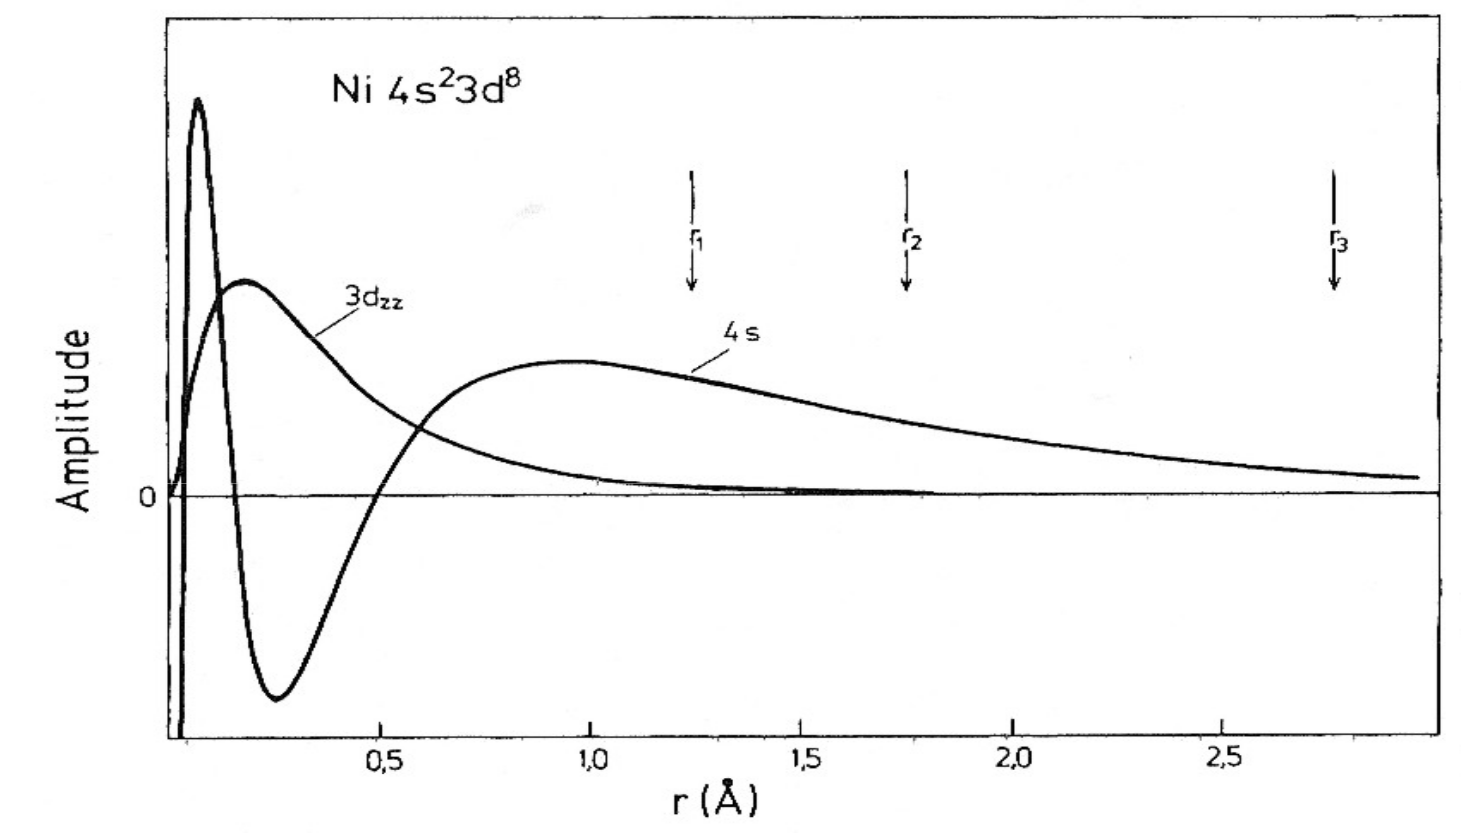
\includegraphics[width=0.8\linewidth]{figures/vl15/ueberlapp_orbitale.png}
		\caption{Überlapp des 3d$_\mathrm{zz}$- und 4s-Orbitals bei Nickel \cite{Ibach}.}
		\label{fig:vl15_ueberlapp_orbitale}
	\end{figure}

\subsubsection{Edelgase und Molekülkristalle, Van-der-Waals-Bindungen}
	Edelgasatome mit vollen Elektronenschalen und Moleküle haben keine freien Valenzelektronen, welche zu einer kovalenten Bindung beitragen könnten und haben keine Tendenz dazu, Elektronen für ionische Bindungen aufzunehmen oder abzugeben. 
	Dennoch sind Edelgase in der Lage dazu, Kristalle zu bilden.
	Die Bindungen enstehen aus Ladungsfluktuationen, welche in einem Atom auftreten. 
	Diese führen zu Dipolmomenten innerhalb eines Atoms. Das entstehende elektrische Feld induziert Dipolmomente in anderen Atomen, wodurch eine induzierte Dipol-Dipol-Wechselwirkung zustande kommt (vgl. \autoref{fig:vl15_abbildung_1}).\\

	\begin{figure}[H]
		\centering
		\incfig{vl15_abbildung_1}
		\caption{Im linken Atom ensteht durch Ladungsfluktuationen ein Dipol $\vec p_1$. Das entstehende Feld $\vec E_\mathrm D$ induziert einen Dipol $p_2$ im rechten Atom.}
		\label{fig:vl15_abbildung_1}
	\end{figure}

	Das Dipolmoment $\Vec{p}_{1}$ eines Moleküls induziert am Ort $\Vec{r}$ das elektrische Feld
	\begin{equation}
		\label{eq:II.2.9}
		\left| \Vec{E}_{0} \right| \sim \frac{\left| \Vec{p}_{1} \right| }{r^3}
	\end{equation}

	und erzeugt im zweiten Molekül mit Polarisierbarkeit $\alpha$ das Dipolmoment 
	\begin{equation}
		\label{eq:II.2.10}
		\left| \Vec{p}_{2} \right| \sim \alpha \left| \Vec{E}_{\mathrm{D}} \right| \sim \frac{\alpha\left| \Vec{p}_1 \right| }{r^3}.
	\end{equation}

	Die potentielle Energie der Dipol-Dipol-Wechselwirkung ist
	\begin{equation}
		\label{eq:II.2.11}
		E_{\mathrm{Dipol}} \sim - \frac{\left| \Vec{p}_{1}  \right| \left| \Vec{p}_{2} \right| }{r^3}.
	\end{equation}
	\eqref{eq:II.2.10} in \eqref{eq:II.2.11} liefert
	\begin{equation}
		\label{eq:II.2.12}
		E_{\text{Dipol}} \sim - \frac{\alpha \left| \Vec{p}_{1} \right| ^2}{r^{6}}.
	\end{equation}

	Zwischen den Atomen wirkt nach dem Pauli-Prinzip eine repulsive Kraft mit $\sim r^{-12}$ (analog zur ionischen Bindung).
	Durch Linearkombination der Coulomb- und Pauli-Interaktion ergibt sich das Lennard-Jones Potential.
	\begin{important}
		\textbf{Lennard-Jones Potential}\\
		\begin{equation}
			\label{eq:II.2.13}
			W_{\text{pot}} = 4 \gamma \left[ \left( \frac{\sigma}{r} \right) ^{12} - \left( \frac{\sigma}{r} \right) ^{6} \right]
		\end{equation}
	\end{important}

	$\gamma$ und $\sigma$ sind empirische Konstanten. Diese Wechselwirkung wird durch das Lennard-Jones-Potential beschrieben und ist auch bekannt als \quickdef{Van-der-Waals-Wechselwirkung}.
	\autoref{fig:vl15_abbildung_2} zeigt den Verlauf des Potentials in Abhängigkeit des Kernabstandes $r$.
	\begin{figure}[H]
		\centering
		\def\svgwidth{.364\columnwidth}
		\subimport{./figures}{vl15_abbildung_2.pdf_tex}
		\caption{Lennard-Jones-Potential $W_\mathrm{pot}$ nach Gleichung \eqref{eq:II.2.13} in Abhängigkeit des Kernabstandes $r$}
		\label{fig:vl15_abbildung_2}
	\end{figure}
	Die Bindungsenergie beträgt ca. \SI{0,1}{\electronvolt \per Atom}. Dies entspricht ca. \SI{10}{\percent} der Gesamtenergie in ionischen Kristallen und \SI{20}{\percent} der Gesamtenergie in Metallen.

\subsubsection{Wasserstoffbrücken}
	Wasserstoffbrücken sind eine Sonderart der ionischen Bindungen.
	Zwei Partner mit hoher Elektronegativität und geringer Koordinationszahl, wie bspw. \ce{HF} oder \ce{H2O}, teilen sich ein Wasserstoffion.\\
	
	\begin{minipage}{0.45\linewidth}
		\begin{figure}[H]
			\centering
			\includegraphics[width=0.7\textwidth]{./figures/vl15_abbildung_3.tikz}
			\caption{Wasserstoffbrücke zwischen zwei Fluoratomen.}
			\label{fig:vl15_abbildung_3}
		\end{figure}
	\end{minipage}
	\hspace{0.1\linewidth}
	\begin{minipage}{0.5\linewidth}
		\autoref{fig:vl15_abbildung_3} zeigt eine Wasserstoffbrücke zwischen zwei Fluoratomen.\\

		Die Bindungsenergie einer Wasserstoffbrücke liegt zwischen \SI{0,1}{\electronvolt} und \SI{0,3}{\electronvolt}. 
	\end{minipage}

\subsection{Kristallstruktur und Symmetrie}
\subsubsection{Translationssymmetrie}
	Kristalle besitzen Symmetrien, welche makroskopisch sichtbar sind. 
	Ein idealer Kristall besteht aus sich periodisch wiederholenden, identischen struktureller Einheiten bzw. Gruppen. 
	Eine strukturelle Einheit wird \quickdef{Basis} genannt und kann von einem einzelnen oder mehreren Atomen gebildet werden. 
	Ein Gitter zusammen mit einer Basis bildet ein Kristallgitter.
\paragraph{Translationsvektoren}
	Mithlfe des Vektors 
	\begin{equation}
		\label{eq:II.2.14}
		\Vec{t} = t_1 \Vec{a}_{1} + t_2 \Vec{a}_{2} + t_3 \Vec{a}_{3}
	\end{equation}
	beschreibt man eine Translation, welche bei einem Gitterpunkt startet und bei einem anderen endet. $\Vec{a}_{i}$ sind primitive Translationsvektoren und $t_{i} \in \mathbb{N}$.
\paragraph{Primitive Gittervektoren}
	{Jeder} Gitterpunkt kann durch eine ganzzahlige Kombination der primitven Gittervektoren erreicht werden. 
	Diese können unterschiedlich gewählt werden, wie in \autoref{fig:vl15_abbildung_4} dargestellt.
	\begin{figure}[H]
		\centering
		\incfig{vl15_abbildung_4}
		\caption{
			$\vec a_i$ und $\vec a'_i$ bilden primitive Gittervektoren des dargestellten Gitters.\\
			$\vec a''_i$ sind nicht primitiv, da Translationen wie $t$ nicht dargestellt werden können.
		}
		\label{fig:vl15_abbildung_4}
	\end{figure}

	Eine \quickdef{primitive elementare Zelle} ist die kleinstmögliche Zelle, welche von primitiven Gittervektoren aufgespannt werden kann. 
	In \autoref{fig:vl15_abbildung_4} ist sie als rote Schattierung zwischen $\vec a_1$ und $\vec a_2$ dargestellt.

\paragraph{Symmetrien im Gitter}
	Ein Kristallgitter kann auf sich selbst abgebildet werden. 
	Dazu werden Symmetrieoperationen wie die Translation im Raum, die Rotation um bestimmte Achsen oder die Spiegelung an Ebenen verwendet.
	Eine \quickdef{Gitterpunktgruppe} umfasst alle Symmetrieoperationen, unter welchen das Gitter invariant ist. Gängige Symmetrien sind:
	\begin{itemize}
		\item die Rotation 
			$
			C = \frac{2\pi}{n}
			$
			mit den Rotationsachsen $n = 1,2,3,4,6$,
		\item die Spiegelung
		\item und die Inversion.
	\end{itemize}
	\begin{verbal}
		Eine Rotation um $C_5={2\pi/}{5}$ ist nicht möglich. 
		Das ist vergleichbar damit, dass sich eine Sammlung an Fünfecken nicht lückenlos aneinanderlegen lässt.\\[1ex]
		Bestimmte Quasikristalle können dennoch $C_5$-symmetrisch sein.
	\end{verbal}
	In \autoref{fig:vl15_wuerfel_symmetrien} sind als Beispiel die Symmetrien eines Würfels dargestellt.
	\begin{figure}[H]
		\centering
		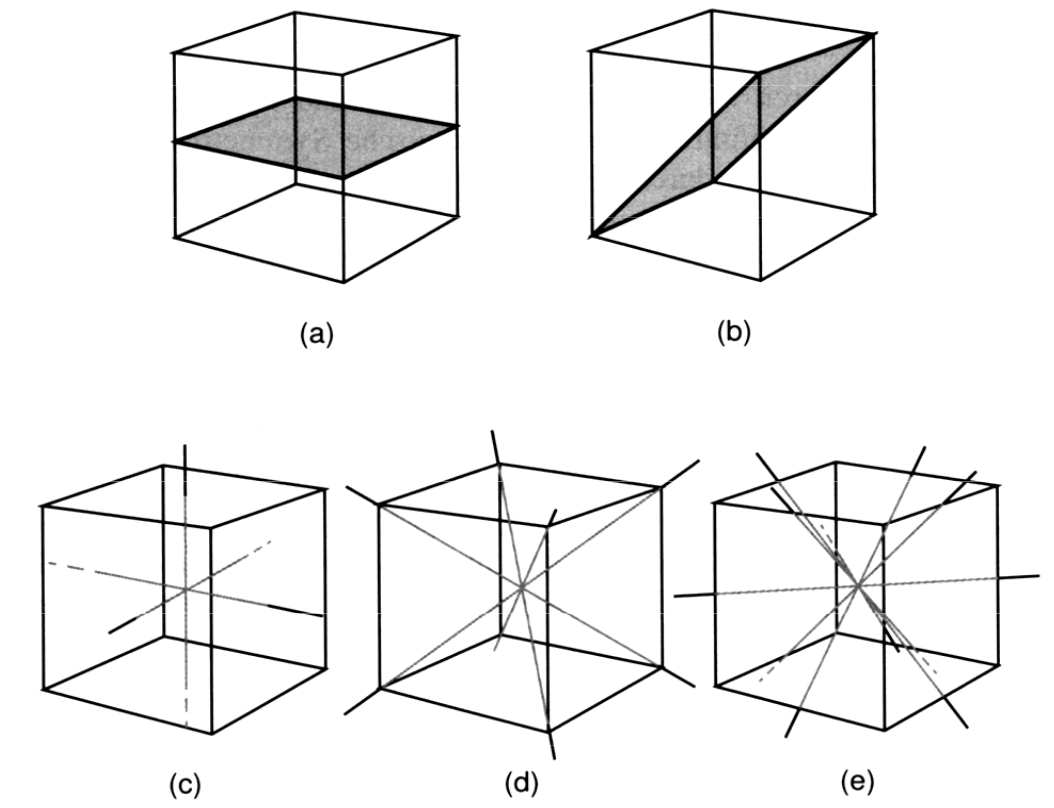
\includegraphics[width = 0.6\linewidth]{figures/vl15/wuerfel_symmetrien.png}
		\caption{Symmetrien eines Würfels \cite{Kittel}. (a) und (b) sind Spiegelungen an Ebenen, (c) bis (e) sind Rotationen um unterschiedlliche Winkel.}
		\label{fig:vl15_wuerfel_symmetrien}
	\end{figure}

\paragraph{Grundlegende Gitter-Typen}
	In drei Dimensionen gibt es 14 verschiedene Gitterarten aufgeteilt in 7 verschiedene Arten an Zellen, welche sich aus den Symmetrien der Punktgruppe ergeben. In \autoref{fig:vl15_gitterarten} sind diese dargestellt.
	\begin{figure}[H]
		\centering
		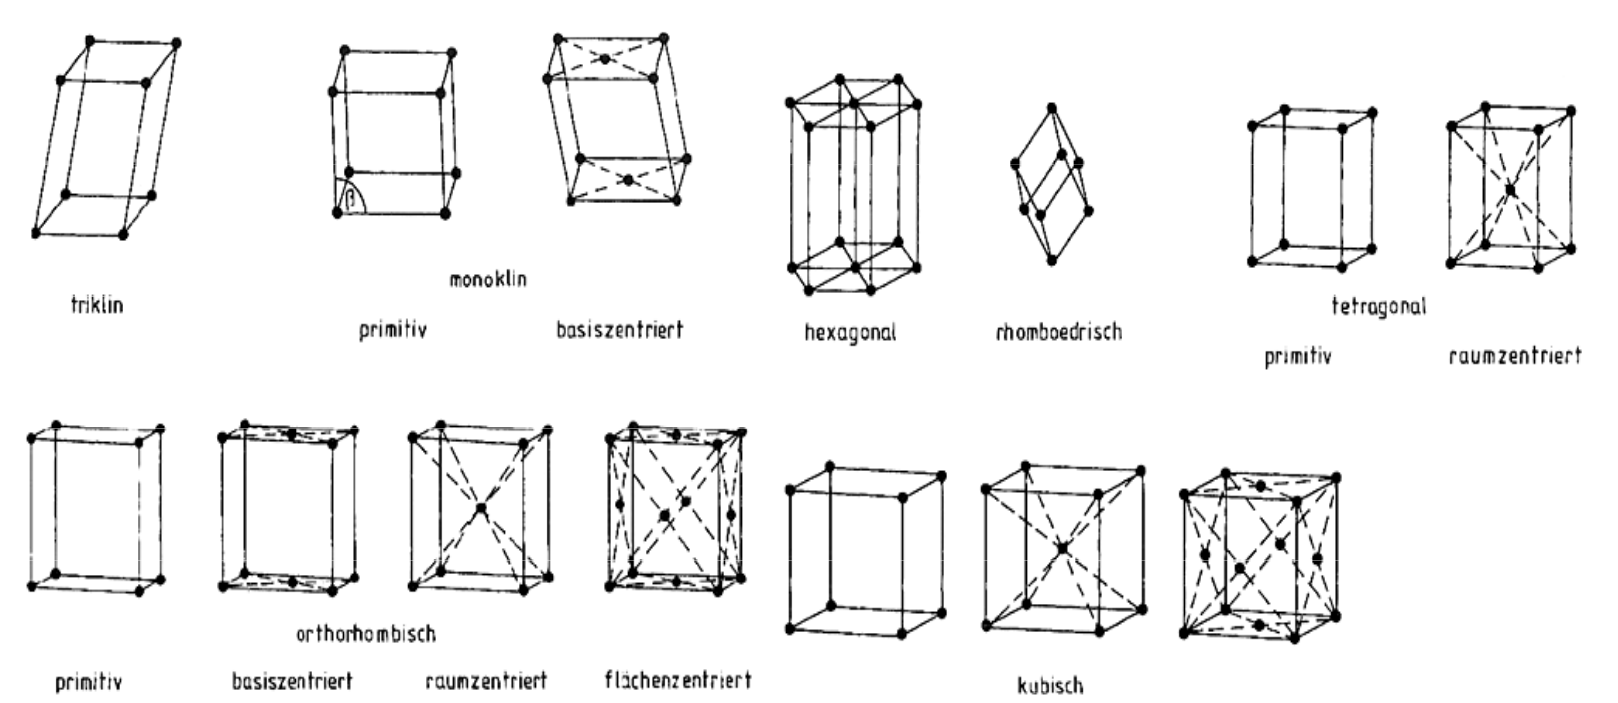
\includegraphics[width=\linewidth]{figures/vl15/gitterarten.png}
		\caption{Gitterarten in drei Dimensionen \cite{Ibach}.}
		\label{fig:vl15_gitterarten}
	\end{figure}

\subsubsection{Punkte, Richtungen und Ebenen in Kristallen}
	Ein \textbf{Punkt} entspricht einem Koeffizient im Translationsgitter (vgl. \autoref{fig:vl15_gitterpunkt}).
	\begin{figure}[H]
		\centering
		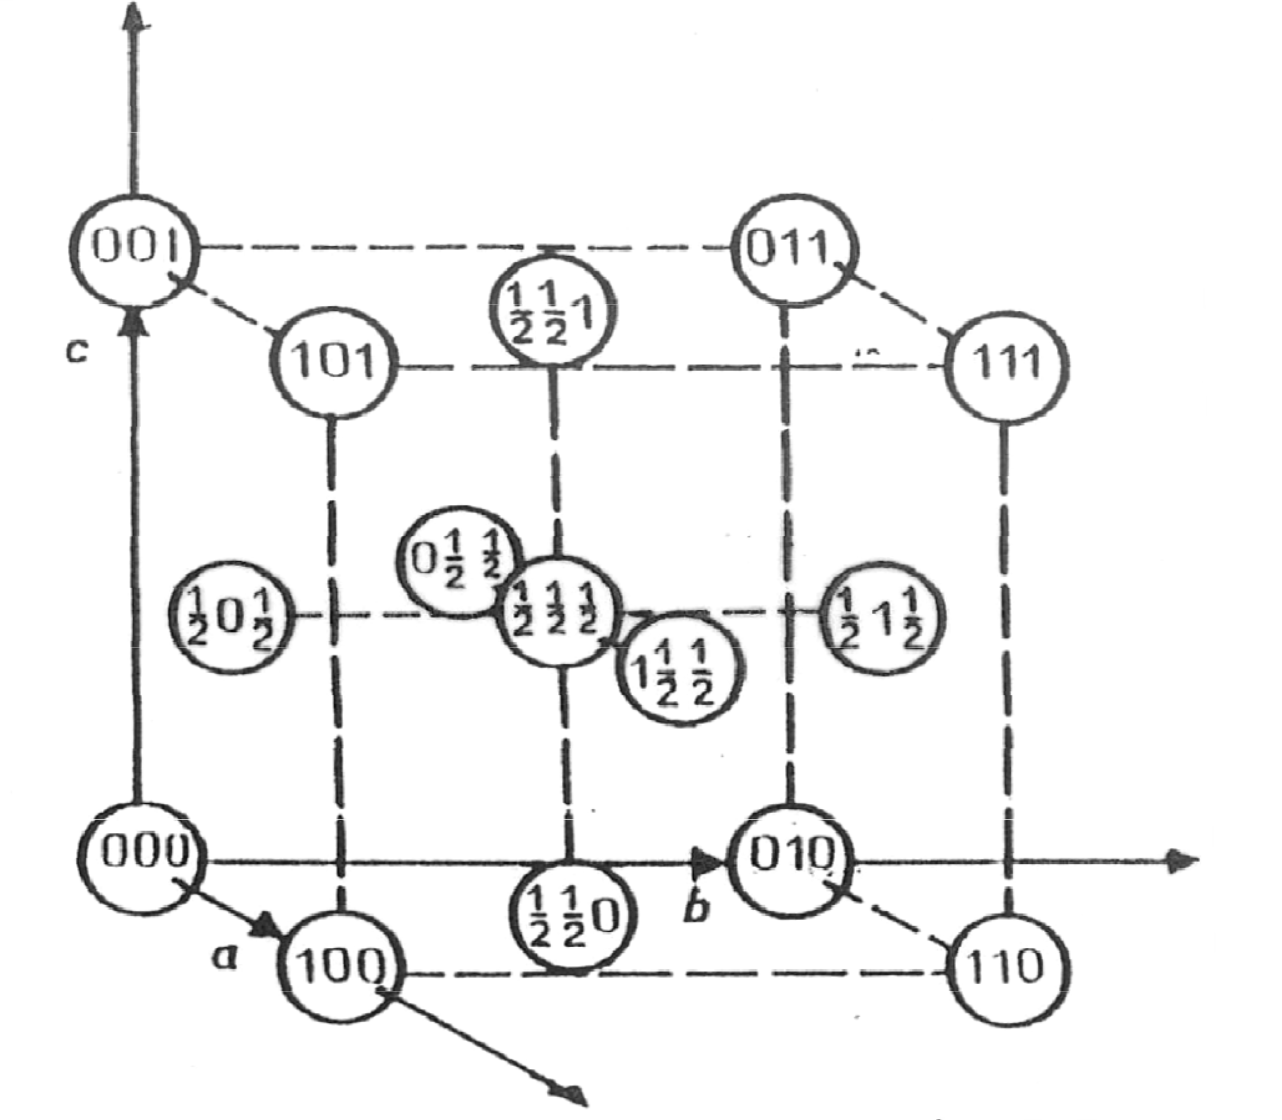
\includegraphics[width=0.5\linewidth]{figures/vl15/gitterpunkte.png}
		\caption{Kennzeichnung der Atompositionen in einer Gitterzelle \cite{Hamann}.}
		\label{fig:vl15_gitterpunkt}
	\end{figure}
	Eine \textbf{Richtung} entspricht der kleinsten ganzzahligen Summe an Gittervektoren. 
	Die Notation und Darstellung der Richtungen ist in \autoref{fig:vl15_gitterrichtung} dargestellt.
	\begin{figure}[H]
		\centering
		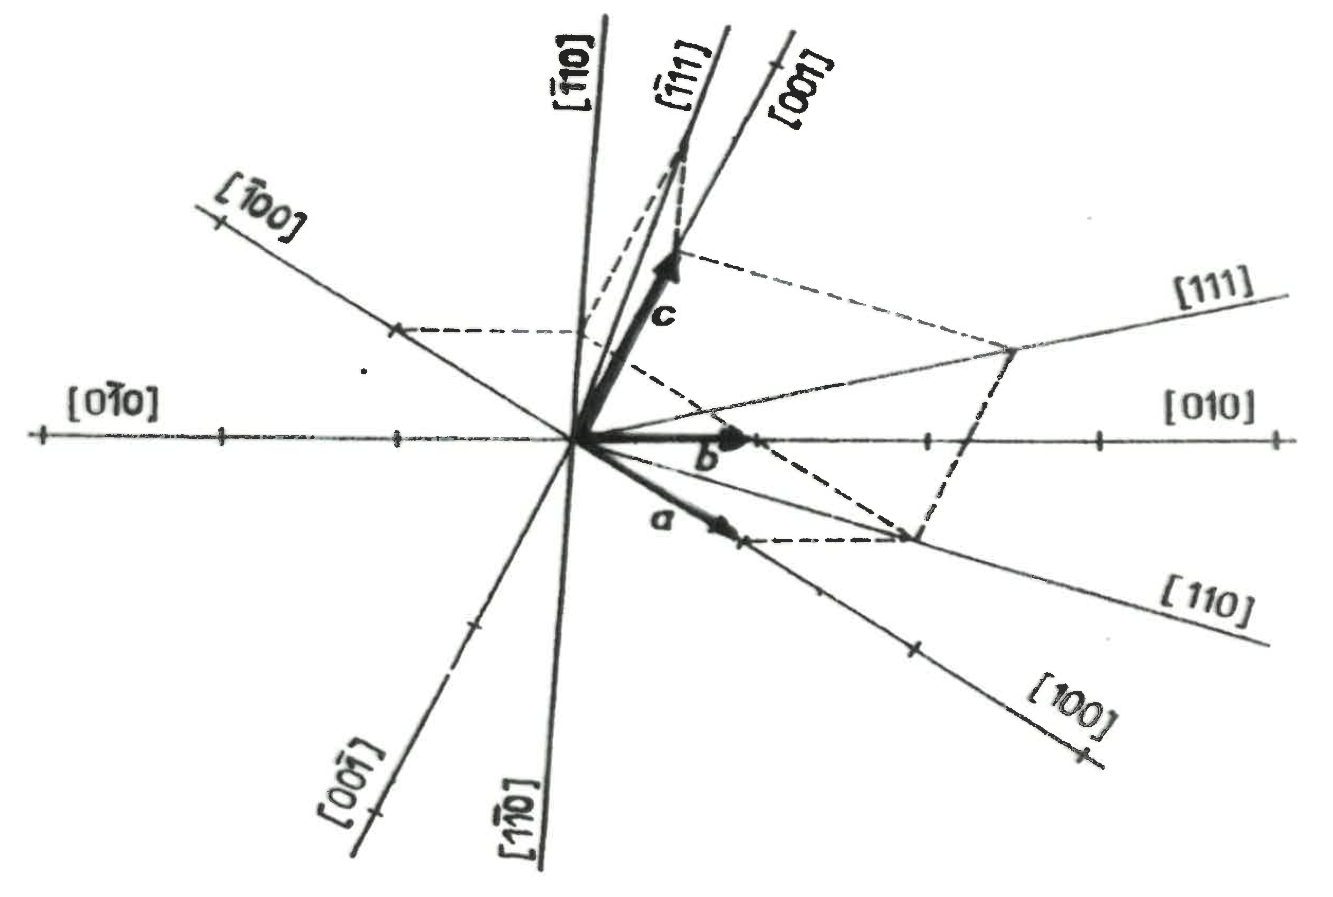
\includegraphics[width=0.5\linewidth]{figures/vl15/gitterrichtung.png}
		\caption{Kennzeichnung der Richtungen im Atomgitter \cite{Hamann}. Negative Zahlen werden mit Strich darüber statt einem Minus gekennzeichnet, also z.B. $[\overline 111]$.}
		\label{fig:vl15_gitterrichtung}
	\end{figure}
	Eine \textbf{Kristallebene} wird definiert durch die Miller-Indizes $(h,k,l)$ definiert, welche sich wie folgt finden lassen:
	\begin{enumerate}
		\item Finde die Schnittpunkte mit den Achsen, angegeben in Vielfachen der Gitterkonstanten $a_1, a_2, a_3$.
			$$
			\text{Beispiel:}\quad 3a_1, \quad 2a_2, \quad 2a_3
			$$ 
		\item 
			\begin{enumerate}
				\item Nehme den Kehrwert
					$$
					\frac{1}{3}, \quad \frac{1}{2}, \quad \frac{1}{2}
					$$ 
				\item Multipliziere mit dem kleinsten gemeinsamen Nenner:
					$$
					(2,3,3)
					$$ 
			\end{enumerate}
			\autoref{fig:vl15_miller_indizes} zeigt die $(2,3,3)$-Ebene.
	\end{enumerate}
	\begin{figure}[H]
		\centering
		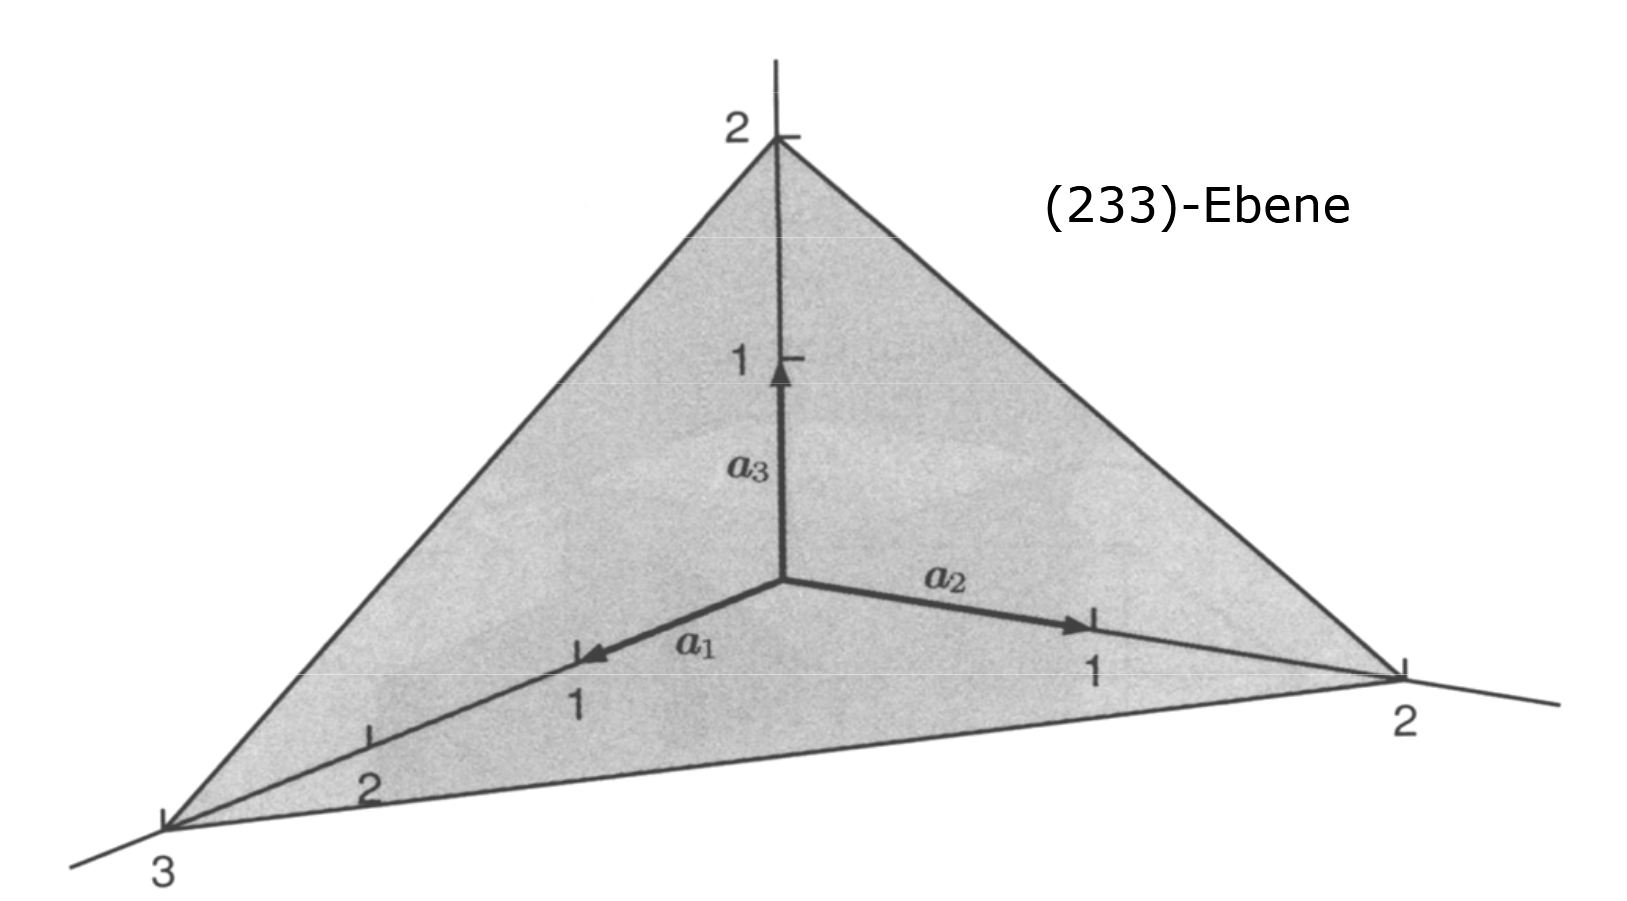
\includegraphics[width=0.5\linewidth]{figures/vl15/miller_indizes.png}
		\caption{$(2,3,3)$-Ebene \cite{Kittel}.}
		\label{fig:vl15_miller_indizes}
	\end{figure}
